\documentclass[a4paper, oneside, zihao = 5, fontset=sourcesans, autoindent = 0em]{ctexbook}

\usepackage{amsmath,dashundergaps, ulem, mwe}
\usepackage[math-style=ISO, bold-style=ISO]{unicode-math} %注意,unicode-math与被其认为过时的bm包不兼容,不要\usepackage{bm}
% TODO:unicode-math较为方便易用和先进,并且较容易由ISO改为GB国标,详情请见
% https://github.com/latexstudio/ChinaThesis/wiki/GB-math
\setmathfont[Scale = 1.1]{Libertinus Math}  

\setmainfont[Scale=1.1, SlantedFont = {Libertinus Serif Italic}]{Libertinus Serif}
\setsansfont{TeX Gyre Heros}
\setmonofont[Scale=1]{Libertinus Mono}



% https://tex.stackexchange.com/questions/279652/macro-like-ignorespaces-for-ignoring-pars
\long\def\eat#1{\ignorepars}
\def\ignorepars{\futurelet\next\ignoreparsA}
\def\ignoreparsA{\ifx\next\par\expandafter\eat\fi}

% 不好的习惯,但却是习俗。
\everymath{\displaystyle}

\dashundergapssetup{
  gap-numbers = false,
  gap-widen = true,
  gap-extend-minimum = 10pt,
  gap-extend-percent = 20,
  teacher-gap-format = underline,
  gap-font = \bfseries \large,
}

\def \ifempty#1{\def\temp{#1} \ifx\temp\empty }
\newcommand{\gapline}[1]{
  \ifanswer
  \dashundergapssetup{teacher-mode = true}
  \else
  \dashundergapssetup{teacher-mode = false}
  \fi%
  \hskip 1pt%
  \ifempty{#1} \gap{\qquad \qquad}
  \else
  \relax\ifmmode \dashundergapssetup{gap-font= \null} \fi \gap{#1} 
  \fi \dashundergapssetup{gap-font= \bfseries \large} \hskip 1pt%
}

\usepackage{geometry}

% TODO:以下为geometry无margin的设定,只适合A4 oneside这样一个页面。以后做其他页面支持时save
% restore各种geometry。

\geometry{%
  includemp = true, % includes the margin notes, \marginparwidth and \marginparsep, into body when calculating horizontal calculation.
  marginparsep = 0cm,
  marginparwidth = 0cm,
  % bindingoffset = 0pt,
  top = 3cm,
  bottom = 3cm,
  % outer = 2cm, % twopage 应当使用inner,outer,而不是left,right
  % inner = 2cm,
  headheight = 6mm,
  headsep = 5mm,
  footskip = 10mm,
  left = 3cm,
  right = 2.5cm, % 如果要为todonotes包要使用的 marginparwidth 留出空间的话,尽量
  %                 % 将其改小,如0.5cm
}

% \addtolength{\oddsidemargin}{-14pt}
% \addtolength{\topmargin}{2pt}

\usepackage{fancyhdr, lastpage}
\pagestyle{fancy} 
\fancyhf{} % clear all header and footer fields
\cfoot{\footnotesize 蛋疼试题\quad 第\,\thepage\,页 \quad (共\pageref{LastPage}页) } %照抄他人
% 代码

\renewcommand{\headrulewidth}{0pt}

\usepackage{enumitem}
% \topsep 列表顶部与之前内容的额外空白,不含 \baselineskip
% \partopsep 如果列表之前是一个空行,列表顶部的额外空白
% \itemsep  列表各项之间额外的垂直空白
% \parsep 一个 item 中,如果分段,段落间额外空白
% \leftmargin 列表与左边距之间的水平距离,值为非负
% \rightmargin 列表与右边距之间的水平距离,值为非负
% \itemindent 每一 item 第一行的缩进
% \listparindent 每一 item 第一行之后各行的缩进
% \labelsep 标签盒子与每一 item 第一行文本之间距离
% \labelwidth 标签盒子的宽度;如果标签过长,这一宽度会自动变大,直到列表的第一行文本为止

% TODO:过时代码,留存Question和Ingroupqu这两个counter,留待以后使用。

\setlist{itemindent = \parindent, listparindent =
  \parindent, %labelindent = \parindent,
  parsep = 0ex, partopsep = 0ex, itemsep = 0em }

\newcounter{Group}
\newcounter{Question}
\newcounter{Ingroupqu}[Group]

\newif\ifbytotal  \bytotalfalse
\bytotaltrue

% TODO:过时代码,留存Question和Ingroupqu这两个counter,留待以后使用。
\newcommand{\addquscounter}{
  \stepcounter{Question}
  \stepcounter{Ingroupqu}
  \ifbytotal
  \renewcommand{\theQuestion}{\arabic{Question}}
  \else 
  \renewcommand{\theQuestion}{\arabic{Ingroupqu}}
  \fi%
}

% TODO:期待enumerate早日完成 \AddEnumerateCounter的新实现。
\newlist{qus}{enumerate}{3}
\setlist[qus]{leftmargin = *, partopsep = 0em, topsep = 0em, 
  parsep = 5pt, itemsep = 0em, leftmargin = 1.4em, listparindent = 0em}

% setlist在目前版本不能叠加效果。
\ifbytotal
  \setlist[qus, 1]{label = {\arabic*}., resume}
\else
  \setlist[qus, 1]{label = {\arabic*}.}
\fi

\setlist[qus, 2]{label = {\arabic*})}
\setlist[qus, 3]{label = {\roman*})}

\newcommand{\group}[1]{
  % 仿section的空间设定。
  % \addvspace{3.5ex plus 1ex minus .2ex}
  \addvspace{3.5ex plus 2ex minus .2ex}
  \stepcounter{Group}
  {\bfseries \chinese{Group}、#1 \par}
  \vskip 0.5em%
}


\makeatletter
\renewcommand*{\title}[1]{\gdef\@title{#1}}

\renewcommand\maketitle{
  \newpage \null%
  \begin{center}%
    {\bfseries\@title \par}%
  \end{center}%
  \par
  \noindent \unskip
}
\makeatother


\newcommand{\fillline}[1]{%
  \hspace*{\fill}\mbox{(\quad#1\quad)}%
}
\usepackage{pifont}
\newif\ifanswer \answerfalse
\answertrue
\newcommand{\dui}{
  \ifanswer \fillline{\ding{52}}
  \else \fillline{\quad}
  \fi
}

\newcommand{\cuo}{
  \ifanswer \fillline{\ding{56}}
  \else \fillline{\quad}
  \fi
}

\newcommand{\choice}[1]{%
  \ifanswer \fillline{\large \bfseries #1}
  \else \fillline{\quad}
  \fi
}

% ------------------------------ 选择题 ----------------------------------%
% 本代码来自于天津大学的TJRSD
% https://github.com/TJRSD/gaokao_exam/blob/master/GEEexam.sty
\usepackage{tasks}%选择题宏包,tasks环境
\settasks{
  counter-format={tsk[A].},
  label-offset={0.4em},
  label-align=left,
  label-width = 1.3em,
  column-sep={2pt},
  item-indent={1pt},
  before-skip={-0.3em},
  after-skip={0em},
  % after-item-skip = 1ex plus 1ex minus 1ex %  default skip
  after-item-skip = 0ex plus 1pt minus 1pt
}


% ------------------------------ 简答题 ----------------------------------%


% TODO: solution,未完成,先占位。 
\newcommand{\solution}[1]{%
  \par
  \ifanswer
  \vspace{1cm}
  \begin{minipage}[t][1cm][t]{0.9\linewidth}
    \large 答案:\par
    #1
  \end{minipage}
  \fi
}

% TODO:subqs subsubqs 先不做,考虑是不是整合所有questions为enumerate,方便嵌套
% 及排版。

\usepackage{tikz}
\usetikzlibrary{shapes,snakes}

% 代码来源于http://www.latexstudio.net/archives/6609.html
% TODO:线条的占用了内部空间,使内部空间不是完全尺寸。
\newcommand{\drawcomposition}[3][0.8]{
  \begin{figure}[!ht]
    \centering
    \begin{tikzpicture}[scale=#1]
      % 画#1条竖线代表单行#1个格
      \foreach \m in {1,2,...,#2}\draw(\m,0) -- (\m,{#3 *1.4 - 0.4});
      % 画#2个横矩形,代表#2行
      \foreach \n in {1,2,..., \the\numexpr#3 }\draw[fill=white,line width=0.4pt](0,{1.4*\n-0.4})rectangle(#2 ,{1.4*\n});
      % 以下#1*#2个方格,如果能定义常量就方便操作了。
      \draw[line width = 0.8pt](0,0)rectangle(#2,{#3 *1.4});
    \end{tikzpicture}
  \end{figure}
}


\title{\zihao{-3}  2018年火星高等学校招生统一考试\\ [-5pt]
  \zihao{-2} \heiti 文理综合}

\usepackage[bodytextleadingratio = 2, restoremathleading = true,
footnoteleadingratio = 1.67]{zhlineskip}

% \usepackage{scalerel}

\begin{document}

\maketitle

{\bfseries \heiti 注意事项}:
\begin{enumerate}
\item 作弊请不要被老师发现。
\item 一旦被发现作弊,不要试图以空口求情或小恩小惠来逃避处罚。
\item “每个人都有一个他无法拒绝的价格。”
\end{enumerate}

\group{判断题:本大题共4小题,每小题5分,共20分。判断下列各题,正确的在题后括号内打\ding{52},错的打\ding{56}。}

\begin{qus}
  
\item 人类一思考,上帝就发笑。\dui
\item 尼采说道:“世上只有一个基督徒,他已经死了”,这句话中所说的“他”是指彼得吗?\cuo
\item 马克思复活后说道:“全世界无产者,原谅我!”,马克思是全盘否定了自己吗?\cuo
\item 你的人生就是一个笑话吗?\dui

\end{qus}

\group{选择题:本大题共4小题,每小题10分,共40分。在每小题给出的四个选项中,只有一项是符合题目要求的。}

\begin{qus}
\item  已知集合~$A=\{x\mid {x-1}<3 \}$,集合~$B=\{y|
  y=x^2+2x+1,x\in\mathbb{R}\}$, 则~$A\cap \complement_U B$~为\choice{C}

  \begin{tasks}(2)
    \task $[\,0,4)$ \task $(-\infty,-2\,]\cup[4,+\infty)$ \task $(-2,0)$
    \task $(0,4)$
  \end{tasks}

\item  若~$a$、$b$~是直线, $\alpha$、$\beta$~是平面,
  则以下命题中真命题是\choice{D}

  \begin{tasks}(1)
    \task 若~$a$、$b$~异面, $a\subset\alpha$,$b\subset\beta$, 且~$a\perp b$, 则~$\alpha\perp\beta$
    \task 若~$a\parallel b$, $a\subset\alpha$, $b\subset\beta$,则~$\alpha\parallel\beta$
    \task 若~$a\parallel \alpha$, $b\subset\beta$, 则~$a$、$b$ 异面
    \task 若~$a\perp b$, $a\perp\alpha$,$b\perp\beta$, 则~$\alpha\perp\beta$
  \end{tasks}

\item 某城市为了解游客人数的变化规律,提高旅游服务质量,收集并整理了2014年1
  月至2016年12月期间月接待游客量(单位:万人)的数据(图1).

  根据图1,下列结论错误的是\choice{A}

  \begin{figure}[!htb]
    \centering
    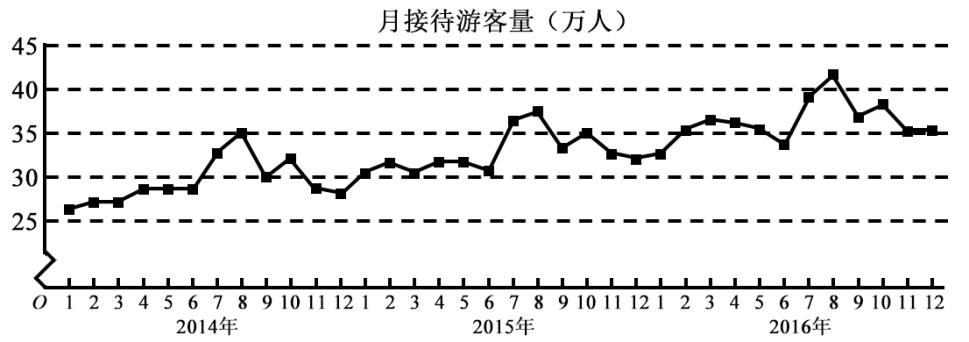
\includegraphics[width=0.8\textwidth]{zxt.jpg}
    \caption{月接待游客量折线图}
    % \label{fig:myphoto}
  \end{figure}%

  \begin{tasks}(1)
    \task 月接待游客量逐月增加 
    \task 年接待游客量逐年增加
    \task 各年的月接待游客量高峰期大致在7,8月份 
    \task 各年1月至6月的月接待游客量相对7月至12月,波动性更小,变化比较平稳 
  \end{tasks}

\item 已知双曲线 $C\colon\,\tfrac{x^2}{a^2}-\tfrac{y^2}{b^2}=1\,(a>0,b>0)$
  的一条渐近线方程为 $y=\tfrac{\sqrt{5}}{2}x$ ,且与椭
  圆$\tfrac{x^2}{12}+\tfrac{y^2}{3}=1$ 有公共焦点,则 $C$ 的方程为\choice{B}

  \begin{tasks}(4)
    \task $\tfrac{x^2}{8}-\tfrac{y^2}{10}=1$ \task $\tfrac{x^2}{4}-\tfrac{y^2}{5}=1$ \task $\tfrac{x^2}{5}-\tfrac{y^2}{4}=1$ \task $\tfrac{x^2}{4}-\tfrac{y^2}{3}=1$ 
  \end{tasks}

\end{qus}

\group{填空题:本题共4小题,每小题5分,共20分。}

\begin{qus}
  
\item 若函数~$f(x)=x^{6m^2-5m-4}\,(m\in\mathbb{Z})$~的图像关于~$y$~轴对称,
  且~$f(2)<f(6)$, 则~$f(x)$~的解析式为 \gapline{$f(x)=x^{-4}$}.

\item 若~$f(x+1)=x^2\,(x\leq0)$, 则$f^{-1}(1)=$ \gapline{$0$}.

\item 已知~$f(x)=1-\textbf{c}_8^1x+\textbf{c}_8^2x^2-\textbf{c}_8^3x^3+\cdots+\textbf{c}_8^8x^8$,
  则~$f\left(\tfrac{1}{2}+\tfrac{\sqrt{3}}{2}\textbf{i}\right)$ 的值是\gapline{$-\tfrac{1}{2}-\tfrac{\sqrt{3}}{2}\textbf{i}$}.

\item 马克思曾说“从前的一切唯物主义(包括费尔巴哈的唯物主义)的主要缺点是:
  对对象、现实、感性,只是从客体的或者直观的形式去理解,而不是把它们当作感性的人
  的活动,当作实践去理解,不是从主体方面去理解。“,所以在他看来,“哲学和对现实世界的研究这两者的关系就像\gapline{手淫}和\gapline{性爱}的关系一样。”

\end{qus}
\clearpage

\group{简答题。}

\begin{qus}
  
\item 已知复数~$z$ 满足:${z}-z^*=\dfrac{10}{1-w\textbf{i}}$(其中~$z^*$
  是~$z$ 的共轭复数).

  \begin{qus}
  \item 求复数 $z$ ;
    \begin{qus}
    \item 我只是占位,显示测试效果的,
    \item 我只是占位,显示测试效果的,
    \item 我只是占位,显示测试效果的,
    \end{qus}
  \item 若复数 $w=\cos\theta+\textbf{i}\sin\theta\,(\theta\in\mathbb{R})$, 求~${z-2}$ 的取值范围.
  \end{qus}

  \solution{
    1) $z=3+4\check{}{i}$

    2) ${z-w}\in[4,6]$
  }

  \vspace{7cm}


\item 已知复数~$z$ 满足:${z}-z^*=\dfrac{10}{1-w\textbf{i}}$(其中~$z^*$
  是~$z$ 的共轭复数).

  \solution{}

  \vfill
\end{qus}

\clearpage

\group{作文题。}

\begin{qus}

\item 阅读下面黑格尔《历史哲学》中的一段话,思考并提出你对这段话的理解。

  \begin{quotation}
    \kaishu 经验或曰历史给我们的教训却是,人民和政府从来就没有从历史学到任
    何东西,从未依照其本应从历史中抽绎出来的教训行事。每个时代都有它特殊的处境,
    都具有一种个别的情况,使它的举动行事,不得不全由自己来考虑、自己来解决。当重
    大事件纷乘交迫的时候,一般笼统的信条毫无裨益。回忆过去的同样情形,也是徒劳无
    功的。一个灰色的回忆不能抗衡``现在''的生动和自由。
  \end{quotation}

  \drawcomposition[0.8]{20}{13}

  \clearpage

  \drawcomposition[0.8]{20}{20}
\end{qus}
\end{document}
